\documentclass[]{article}
\newcommand{\FileDepth}{../../..}
\usepackage[letterpaper, landscape, margin=0.5cm]{geometry}
\usepackage[T1]{fontenc}
\usepackage{textcomp}%Not strictly necessary, but gives \textmu command for "micro."
\usepackage{fancyhdr}
\usepackage{amsmath}
\usepackage{amssymb}
\usepackage{graphicx}
\usepackage{xcolor}
\usepackage{tikz}
\usetikzlibrary{calc}
\usepackage[shortlabels]{enumitem}
\usepackage{multicol}
\usepackage{vwcol}
\usepackage{hyperref}
\usepackage{wrapfig}
%opening
\newcommand{\SecType}{L}
\newcommand{\Week}{14}
\title{PH 211 Lecture \Week}
\author{Benjamin Bauml}
\date{Summer 2024}

\newcommand{\Purpose}{4}
\newcommand{\DefOnly}{0}

\input{\FileDepth/Formats/Assignment20240614.tex}
\usepackage[absolute]{textpos}
% This package relies on Assignment Format 2024-06-14 or later to work. It is recommended that the Purpose and DefOnly commands be given as such:
%\newcommand{\Purpose}{4}
%\newcommand{\DefOnly}{0}
% Activities need to be entered outside of the TeacherMargin and PresentSpace environments, otherwise they will be defined only locally. They can even go in the preamble.
\newenvironment{TeacherMargin}{\begin{textblock*}{10.8cm}(0.5cm,0.5cm)
\small}{\end{textblock*}
\hspace{0.1cm}}
\newenvironment{PresentSpace}{\begin{textblock*}{0.3cm}(26.85cm,9.35cm)
--
\end{textblock*}
\begin{textblock*}{15.6cm}(11.8cm,0.5cm)
\begin{Repurpose}{1}
\Large}{\end{Repurpose}
\end{textblock*}
\hspace{0.1cm}}

\newcommand{\FBDaxes}[4][2]{
	\begin{scope}[shift={(#2)},rotate=#3]
		% x-axis
		\draw[thick,->] (-#1,0) -- (#1,0);
		\node[anchor=west] at (#1,0) {$x$};
		% y-axis
		\draw[thick,->] (0,-#1) -- (0,#1);
		\node[anchor=south] at (0,#1) {$y$};
		\coordinate (#4) at (0,0);
	\end{scope}
}
\newcommand{\FBDvectorMA}[4]{
	\begin{scope}[shift={(#1)}]
		\coordinate (#4tip) at ({#2*cos(#3)},{#2*sin(#3)});
		\draw[ultra thick,blue,->] (#1) -- (#4tip);
	\end{scope}
}
\newcommand{\FBDvectorXY}[3]{
	\begin{scope}[shift={(#1)}]
		\coordinate (#3tip) at (#2);
		\draw[ultra thick,blue,->] (0,0) -- (#3tip);
	\end{scope}
}
\newcommand{\FBDdot}[1]{
	\filldraw[black] (#1) circle (3pt);
}
\newcommand{\FBDbox}[5][1]{
	\begin{scope}[shift={(#2)},rotate=#3]
		\filldraw[color=black,fill=white,thick] ({-#1/2},{#1/2}) -- ({-#1/2},{-#1/2}) -- ({#1/2},{-#1/2}) -- ({#1/2},{#1/2}) -- cycle;
		% Left side coordinates
		\coordinate (#4ltq) at ({-#1/2},{#1/4});
		\coordinate (#4lcent) at ({-#1/2},0);
		\coordinate (#4lbq) at ({-#1/2},{-#1/4});
		% right side coordinates
		\coordinate (#4rtq) at ({#1/2},{#1/4});
		\coordinate (#4rcent) at ({#1/2},0);
		\coordinate (#4rbq) at ({#1/2},{-#1/4});
		% top coordinates
		\coordinate (#4tlq) at ({-#1/4},{#1/2});
		\coordinate (#4tcent) at (0,{#1/2});
		\coordinate (#4trq) at ({#1/4},{#1/2});
		% bottom coordinates
		\coordinate (#4blq) at ({-#1/4},{-#1/2});
		\coordinate (#4bcent) at (0,{-#1/2});
		\coordinate (#4brq) at ({#1/4},{-#1/2});
		% corners
		\coordinate (#4tl) at ({-#1/2},{#1/2});
		\coordinate (#4tr) at ({#1/2},{#1/2});
		\coordinate (#4bl) at ({-#1/2},{-#1/2});
		\coordinate (#4br) at ({#1/2},{-#1/2});
		\node at (0,0) {#5};
	\end{scope}
}
%\newcommand{\MVec}[3][0]{%Creates a momentum vector of length #3 centered at #2 and rotated #1 degrees counterclockwise.
	\begin{scope}[rotate=#1,shift={(#2)}]
		\draw[->,thick] ({-#3/2},0) -- ({#3/2},0);
	\end{scope}
}
\newcommand{\MDot}[1]{%Creates a dot at #1 to represent a zero vector.
	\filldraw (#1) circle (1pt);
}
\newcommand{\MVDRows}[2][4.5]{%Creates the rows (initial, delta, final) of a momentum vector diagram. The optional argument determines the width of the table, and defaults to a good length for three columns (two objects and the total system). The non-optional argument gives a coordinate name (not displayed) to the diagram.
	\begin{scope}
		%\draw[thick] (0,5.5) -- (0,0);
		\draw[thick] (-1,4.5) -- (#1,4.5);
		\node at (-0.5,3.75) {$\vec{p}_{i}$};
		\draw[thick] (-1,3) -- (#1,3);
		\node at (-0.5,2.25) {$\Delta\vec{p}$};
		\draw[thick] (-1,1.5) -- (#1,1.5);
		\node at (-0.5,0.75) {$\vec{p}_{f}$};
		\coordinate (#2) at (0,5);
	\end{scope}
}
\newcommand{\MVDCol}[4][0.75]{%Creates a column for an object in a momentum vector diagram. The first (non-optional) argument is the coordinate name (not displayed) of the column, while the second is the displayed column header. The first argument also names the three entries down the column. The third argument anchors the column, so it should either be the coordinate name of the MVD (for the first column) or the coordinate name of the previous column. The optional argument indicates how far the center of the column should be from the previous column's edge, and defaults to 0.75.
	\begin{scope}[shift={(#4)}]
		\node at (#1,0) {#3};
		%\draw[thick] ({#1*2},0.5) -- ({#1*2},-5);
		\draw[thick] (0,0.5) -- (0,-5);
		\coordinate (#2init) at (#1,-1.25);
		\coordinate (#2delt) at (#1,-2.75);
		\coordinate (#2fin) at (#1,-4.25);
		\coordinate (#2) at ({#1*2},0);
	\end{scope}
}

%\input{\FileDepth/Activities/Activity_One/Activity_One.tex}
%\input{\FileDepth/Activities/Activity_Two/Activity_Two.tex}

\begin{document}
\begin{TeacherMargin}

\end{TeacherMargin}
\begin{PresentSpace}
\begin{center}
	\huge Lecture \Week: Dynamics of Related Systems
\end{center}
\vspace{0.5cm}
\underline{Warm-Up Activity} \\
Is the acceleration of block B greater than, less than, or equal to the acceleration of block A?
%\begin{multicols}{2}
\begin{enumerate}[(A)]
	\item Greater than
	\item Less than
	\item Equal to
	\item Not enough information
\end{enumerate}
%\end{multicols}
\end{PresentSpace}
\begin{textblock*}{5cm}(19cm,4.5cm)
	\begin{center}
		\Large
		\begin{tikzpicture}
			\foreach \n in {0,4.5}
				\draw[thick,color=black,fill=gray,shift={(\n,0)}] (0,0) rectangle (2.5,2.5);
			\foreach \n in {0,4.5}
				\draw[thick,shift={(\n,0)}] (0,2.5) rectangle (1,3.5);
			\foreach \n in {0,4.5}
				\draw[thick,shift={(\n,0)}] (2.7,2.7) circle (0.3);
			\foreach \n in {0,4.5}
				\draw[thick,shift={(\n,0)}] (1,3) -- (2.7,3) arc (90:0:0.3) -- (3,1.25);
			\node at (0.5,3) {A};
			\node at (5,3) {B};
			\draw[thick] (2.7,1.25) rectangle (3.3,0.65);
			\draw[thick,shift={(4.5,0)}] (3,1.25) -- (3,0.65);
			\node[rotate=160] at (7.75,0.65) {\includegraphics[scale=0.75]{KnightHand}};
			\node[anchor=east] at (3.3,-0.5) {Weight = 10 N};
			\node[anchor=east] at (7.8,-0.5) {Tension = 10 N};
		\end{tikzpicture}
	\end{center}
\end{textblock*}
\newpage
\begin{TeacherMargin}

\end{TeacherMargin}
\begin{PresentSpace}
\vspace{-10pt}
\section*{A Model for Interactions}
\vspace{-10pt}
\begin{itemize}
	\item Quantities
	\begin{itemize}
		\item Mass \quad $m$ \qquad \textbf{--} Force \quad $\vec{F}$
		%\item Force \quad $\vec{F}$
	\end{itemize}
	\item Laws
	\begin{itemize}
		\item Net force is proportional to acceleration: \\
		$\vec{F}^{net}=m\vec{a}$
		\item Forces come in pairs: $\vec{F}_{AB} = -\vec{F}_{BA}$
	\end{itemize}
	\item Assumptions
	\begin{itemize}
		\item We can treat multiple objects as a system.
		\item All forces act as if on the center of the system.
	\end{itemize}
\end{itemize}
\end{PresentSpace}
\newpage
\begin{TeacherMargin}

\end{TeacherMargin}
\begin{PresentSpace}
\vspace{-10pt}
\section*{Types of Forces}
\vspace{-10pt}
\begin{itemize}
	\item Gravity \qquad \qquad \qquad \qquad $\vec{F}^{g}_{AB} = m_{A}\vec{g}_{B}$
	\begin{itemize}
		\item Newtonian \qquad\ $\vec{g}_{B} = G\frac{M_{B}}{r^{2}}(-\hat{r})$, $G = 6.67408\times10^{-11}\text{ N}\cdot\text{m}^{2}/\text{kg}^{2}$
		\item Near-Earth \qquad $\vec{g}_{E} = g(-\hat{y}),\ g=9.81\frac{\text{m}}{\text{s}^{2}} \approx 10\frac{\text{m}}{\text{s}^{2}}$
	\end{itemize}
	\item Normal \qquad $\vec{F}^{N}$ always $\bot$; varies in magnitude
	\item Tension \qquad $\vec{F}^{T}$ uniform (massless, inextensible rope)
	\item Spring \qquad $\vec{F}^{S}=-k(\vec{x}-\vec{x}_{eq})$
	\item Friction
	\begin{itemize}
		\item Static Friction \qquad $F^{sf}\leq\mu_{s}|\vec{F}^{N}|$
		\item Kinetic Friction \qquad $F^{kf}=\mu_{k}|\vec{F}^{N}|$
	\end{itemize}
\end{itemize}
\end{PresentSpace}
\newpage
\begin{TeacherMargin}

\end{TeacherMargin}
\begin{PresentSpace}
\vspace{-10pt}
\section*{Newton's 3rd Law of Motion}
\vspace{-10pt}
\begin{itemize}
	\item If A exerts a force on B, then B exerts a force of the same magnitude on A in the opposite direction:
	\[
	\vec{F}^{t}_{AB} = -\vec{F}^{t}_{BA}
	\]
	\item These two forces make a \textit{Newton's 3rd law pair}, or an \textit{action-reaction pair}.
	\item 3rd law pair forces\dots
	\begin{itemize}
		\item are the same type of force;
		\item appear on different free body diagrams.
	\end{itemize}
\end{itemize}
\end{PresentSpace}
\newpage
\begin{TeacherMargin}
\noindent First, we know from the ideal rope and ideal pulley assumptions that the tension is uniform throughout the rope, so we can define $F^{T}_{AR} = F^{T}_{WR} = F^{T}$. \\

\noindent Case B is fairly straightforward.
\begin{center}
	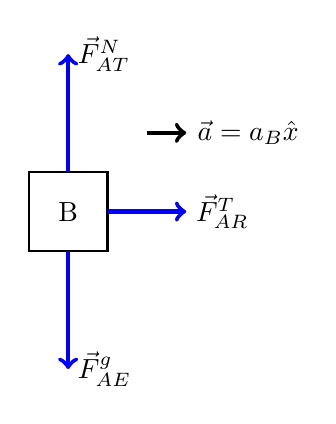
\begin{tikzpicture}
		\FBDbox{0,0}{0}{B}{B}
		\FBDvectorXY{Btcent}{0,1.5}{FNAT}
		\node[anchor=west] at (FNATtip) {$\vec{F}^{N}_{AT}$};
		\FBDvectorXY{Bbcent}{0,-1.5}{FGAE}
		\node[anchor=west] at (FGAEtip) {$\vec{F}^{g}_{AE}$};
		\FBDvectorXY{Brcent}{1,0}{FTAR}
		\node[anchor=west] at (FTARtip) {$\vec{F}^{T}_{AR}$};
		\draw[ultra thick,->] (1,1) -- (1.5,1) node[anchor=west] {$\vec{a} = a_{B}\hat{x}$};
	\end{tikzpicture}
\end{center}
We can see that $\vec{F}^{net} = \vec{F}^{T}_{BR}$, therefore $a_{B} = \frac{F^{T}_{BR}}{m_{B}}$. \\

\noindent In case A, we have two free-body diagrams, one for B and one for the weight W:
\begin{center}
	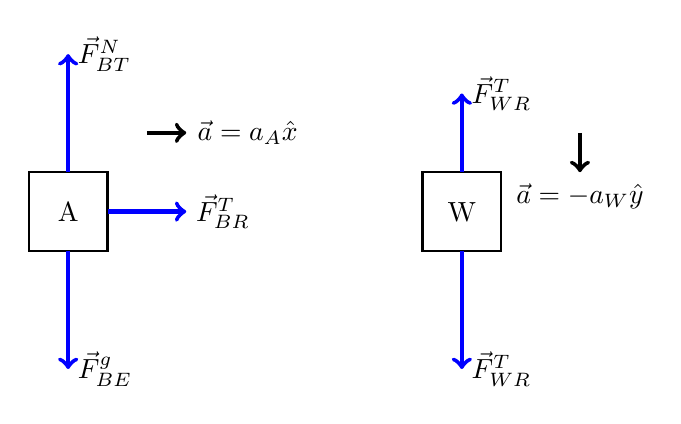
\begin{tikzpicture}
		\FBDbox{0,0}{0}{B}{A}
		\FBDvectorXY{Btcent}{0,1.5}{FNAT}
		\node[anchor=west] at (FNATtip) {$\vec{F}^{N}_{BT}$};
		\FBDvectorXY{Bbcent}{0,-1.5}{FGAE}
		\node[anchor=west] at (FGAEtip) {$\vec{F}^{g}_{BE}$};
		\FBDvectorXY{Brcent}{1,0}{FTAR}
		\node[anchor=west] at (FTARtip) {$\vec{F}^{T}_{BR}$};
		\draw[ultra thick,->] (1,1) -- (1.5,1) node[anchor=west] {$\vec{a} = a_{A}\hat{x}$};
		\FBDbox{5,0}{0}{W}{W}
		\FBDvectorXY{Wtcent}{0,1}{FTWR}
		\node[anchor=west] at (FTWRtip) {$\vec{F}^{T}_{WR}$};
		\FBDvectorXY{Wbcent}{0,-1.5}{FGWE}
		\node[anchor=west] at (FGWEtip) {$\vec{F}^{T}_{WR}$};
		\draw[ultra thick,->] (6.5,1) -- (6.5,0.5) node[anchor=north] {$\vec{a} = -a_{W}\hat{y}$};
	\end{tikzpicture}
\end{center}
We still have $F^{T}= m_{A}a_{A}$, just like before. On the weight, Newton's second law tells us that $F^{T} = m_{W}g-m_{W}a_{A}$ (both have the same acceleration, as they are attached). Combining these, we have
\begin{align*}
	m_{W}g-m_{W}a_{A} & = m_{A}a_{A} \\
	m_{W}g & = a_{A}(m_{A}+m_{W}) \\
	a_{A} & = \frac{m_{W}g}{m_{A}+m_{W}}
\end{align*}
We are given that $m_{W}g=10$ N in case A, and $F^{T}_{BR}=10$ N in case B. As such, it can be seen that $a_{A} < a_{B}$. \\

\noindent Conceptually, the only way the blocks could tie is if they had the same acceleration, which would mean having the same tension in cases A and B. However, if the rope in A had 10 N of tension, then the forces on the weight would be balanced (10 N tension versus 10 N gravity) and the weight itself would not accelerate. We need the forces on the weight to be unbalanced, which means the tension must be smaller than the force of gravity, and A won't be pulled as hard.
\end{TeacherMargin}
\begin{PresentSpace}
\vspace{-10pt}
\section*{L\Week-1: The Block Race}
\vspace{-10pt}
Below left, block A is accelerated across a frictionless table by a hanging 10 N weight. Below right, an identical block B is accelerated by a constant 10 N tension in the string. Neglect friction in both cases.
\begin{enumerate}[(A)]
	\item Draw free-body diagrams for each situation.
	\item Indicate the direction of the \\
	acceleration for each object.
	\item Solve for the acceleration \\
	of each block.
\end{enumerate}
\end{PresentSpace}
\begin{textblock*}{5cm}(19cm,4.5cm)
\begin{center}
	\Large
	\begin{tikzpicture}
		\foreach \n in {0,4.5}
		\draw[thick,color=black,fill=gray,shift={(\n,0)}] (0,0) rectangle (2.5,2.5);
		\foreach \n in {0,4.5}
		\draw[thick,shift={(\n,0)}] (0,2.5) rectangle (1,3.5);
		\foreach \n in {0,4.5}
		\draw[thick,shift={(\n,0)}] (2.7,2.7) circle (0.3);
		\foreach \n in {0,4.5}
		\draw[thick,shift={(\n,0)}] (1,3) -- (2.7,3) arc (90:0:0.3) -- (3,1.25);
		\node at (0.5,3) {A};
		\node at (5,3) {B};
		\draw[thick] (2.7,1.25) rectangle (3.3,0.65);
		\draw[thick,shift={(4.5,0)}] (3,1.25) -- (3,0.65);
		\node[rotate=160] at (7.75,0.65) {\includegraphics[scale=0.75]{KnightHand}};
		\node[anchor=east] at (3.3,-0.5) {Weight = 10 N};
		\node[anchor=east] at (7.8,-0.5) {Tension = 10 N};
	\end{tikzpicture}
\end{center}
\end{textblock*}
\newpage
\begin{TeacherMargin}
	
\end{TeacherMargin}
\begin{PresentSpace}
\section*{Main Ideas}
\begin{itemize}
	\item The magnitude of kinetic friction can be modeled as directly proportional to the magnitude of the normal force.
	\item Newton's 3rd law of motion can be used to relate the forces acting on \textit{different} systems.
\end{itemize}
\end{PresentSpace}
\end{document}